\documentclass[DynamicalBook]{subfiles}
\begin{document}
%




\setcounter{chapter}{0}%Just finished 0.


%------------ Chapter ------------%
\chapter{Deterministic Systems}

\section{Introduction}

Here's a basic fact of life: \emph{things change}. And how things change most
often depends on how they currently are. This is the basic idea underlying all the various notions of \emph{dynamical
  system} that we will see in this book.

\begin{informal}
  A \emph{dynamical system} consists of:
  \begin{itemize}
  \item a notion of how things are, called the \emph{state}, and
  \item a notion of how things will change given how they are, called the \emph{dynamics}.
  \end{itemize}
  The dynamics of a system might also depend on some free \emph{parameters}, and
  we will often only be interested in some particular \emph{variables} of the
  state. 
\end{informal}

In this chapter, we will see this idea in its
most distilled form: we will know exactly how things are, and what they will be
like next. That is, we'll be focusing on \emph{deterministic} dynamical systems,
whose time steps forward in \emph{discrete} increments.


A paradigmatic example of this sort of dynamical system is a clock.
\[
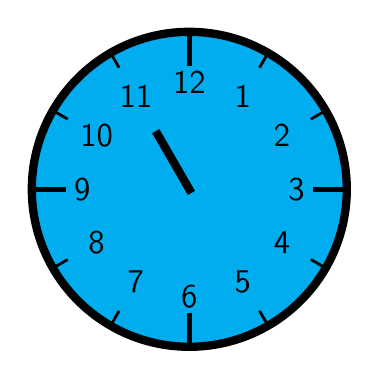
\begin{tikzpicture}[line cap=rect,line width=3pt]
\filldraw [fill=cyan] (0,0) circle [radius=2cm];
\foreach \angle [count=\xi] in {60,30,...,-270}
{
  \draw[line width=1pt] (\angle:1.8cm) -- (\angle:2cm);
  \node[font=\large] at (\angle:1.36cm) {\textsf{\xi}};
}
\foreach \angle in {0,90,180,270}
  \draw[line width=2pt] (\angle:1.6cm) -- (\angle:2cm);
\draw (0,0) -- (120:0.8cm);
\end{tikzpicture}
\]

Suppose that our clock has just an hour hand for now. Then we may collect all
the way things can be for the clock into a set of hours:
$$\Set{Hours} := \{1, 2, 3, 4, 5, 6, 7, 8, 9, 10, 11, 12\}.$$

The set $\Set{Hours}$ is the set of \emph{states} of our clock system. If we know what hour it is, we also know what hour is coming next. So, this system has the following dynamics:
%
% :CUSTOM-ID: problem-with-drawing-mapsto-nicely
%
\begin{align*}
  \fun{tick} : \Set{Hours} &\to \Set{Hours} \\
                t &\mapsto \begin{cases} t + 1 &\mbox{if $t < 12$}\\ 1 &\mbox{if $t = 12$}  \end{cases}
\end{align*}

Here's a sample of the dynamics of the clock. Say we started at 3 o'clock:
$$3 \xmapsto{\fun{tick}} 4 \xmapsto{\fun{tick}} 5 \xmapsto{\fun{tick}} 6
\xmapsto{\fun{tick}} \cdots$$

Not the most dynamic of systems, but we have to start somewhere. If we want to
refer to the whole system at once, we can box it up and write it like this:

\begin{equation}\label{eqn.clock_system_box}\tag{Clock System}
\begin{tikzpicture}[oriented WD, bbx = 1cm, bby =.5cm, bb min width=1cm, bb port length=4pt, bb port sep=1]
	\node[bb={0}{1}] (X) {$\Sys{Clock}$};
	\draw[label] 
		node [right=2pt of X_out1] {$\Set{Hours}$}
		;
\end{tikzpicture}
\end{equation}

We imagine that the clock is going about its business inside the box, and
that is shows the hour it is currently displaying on the outgoing wire.

One issue with our clock is that it doesn't tell us whether it is morning or
evening. Being morning or evening is its own way that things might be, and we
can see it as its own dynamical system. We might imagine a little addition to
our clock that reads $\const{a.m.}$ or $\const{p.m.}$:
\begin{equation}\label{eqn.whole_clock}
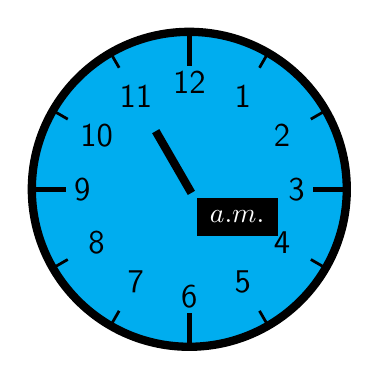
\begin{tikzpicture}[line cap=rect,line width=3pt]
\filldraw [fill=cyan] (0,0) circle [radius=2cm];
\foreach \angle [count=\xi] in {60,30,...,-270}
{
  \draw[line width=1pt] (\angle:1.8cm) -- (\angle:2cm);
  \node[font=\large] at (\angle:1.36cm) {\textsf{\xi}};
}
\foreach \angle in {0,90,180,270}
  \draw[line width=2pt] (\angle:1.6cm) -- (\angle:2cm);
\draw (0,0) -- (120:0.8cm);
\node[draw, fill] at (330:.7cm) {$\color{white}\const{a.m.}$};
\end{tikzpicture}
\end{equation}

We can see this little addition as a system in its own right; it is the system
of $\const{a.m.}/\const{p.m.}$. The states of this system are
$$\Set{Meridien} = \{\const{a.m.}, \const{p.m.}\}.$$
But this time, knowing how they are going to change also requires us to know the
hour:
\begin{align*}
  \fun{next} : \Set{Meridien} \times \Set{Hours} &\to \Set{Meridien} \\
               (\const{a.m.}, t) &\mapsto \begin{cases} \const{p.m.} &\mbox{if $t = 11$}\\ \const{a.m.} &\mbox{otherwise}  \end{cases} \\
               (\const{p.m.}, t) &\mapsto \begin{cases} \const{a.m.} &\mbox{if $t = 11$}\\ \const{p.m.} &\mbox{otherwise}  \end{cases}
\end{align*}
If it is $\const{a.m.}$ and the clock reads 8, then it will still be
$\const{a.m.}$; but if it is $\const{a.m.}$ and the clock reads 11, then it will
switch on the next hour to $\const{p.m.}$.

The thing to note about the dynamics of the $\const{a.m.}/\const{p.m.}$ system
is that they depend on what hour it is. The hour is a \emph{parameter} for the
dynamics of this system. We can draw this system as a box like this:
\begin{equation}\label{eqn.am_pm_system_box}
\begin{tikzpicture}[oriented WD, bbx = 1cm, bby =.5cm, bb min width=1cm, bb port length=4pt, bb port sep=1]
	\node[bb={1}{1}] (X) {$\Sys{a.m./p.m.}$};
	\draw[label] 
		node [left=2pt of X_in1] {$\Set{Hours}$}
		node [right=2pt of X_out1] {$\Set{Meridien}$}
		;
\end{tikzpicture}
\end{equation}
We have the $\Set{Meridien}$ wire coming out, which carries the information of
whether it is $\const{a.m.}$ or $\const{p.m.}$, just like the clock. But we also
have a wire coming in, which carries the hour that we need as a parameter for
our dynamics.


We can now express our whole clock (\ref{eqn.whole_clock}) by wiring together
our bare clock and the $\const{a.m.}/\const{p.m.}$ system:

\begin{equation}\label{eqn.clock_system_box}
\begin{tikzpicture}[oriented WD, bbx = .3cm, bby =.3cm, bb min width=.5cm, bb port length=2pt, bb port sep=1]
	\node[bb={1}{1}] (X1) {$\Sys{a.m./p.m.}$};
  	\node[bb={0}{1}, below=2 of X1] (X2) {$\Sys{Clock}$};
	\node[bb={0}{2}, fit={($(X1.north west)+(-2,1)$) ($(X1.north east)+(2,1)$) ($(X2.south)+(0,-3)$)}] (Y) {};
  \node[above=0pt of Y.south] (Label) {$\Sys{ClockWithDisplay}$};
	\draw (X1_out1) to (Y_out1);
  \draw let \p1=(X1.south west), \p2=(X2.north east), \n1=\bbportlen, \n2=\bby in
    (X2_out1) to[in=0] (\x2 + \n1, \y2 + \n2) -- (\x1 - \n1, \y2 + \n2) to[out=180] (X1_in1);
  \draw (X2_out1) to (Y_out2);
	\draw[label] 
		node [right=2pt of Y_out1] {$\Set{Meridien}$}
		node [right=2pt of Y_out2] {$\Set{Hours}$}
		;
\end{tikzpicture}
\end{equation}

This system has states
$$\Set{HoursWithDisplay} := \Set{Hours} \times \Set{Meridien}$$
consisting of a pair $(11, \const{a.m.})$ of an hour and a meridien reading.
They update in a combined way, by using the hour shown on the clock face as the
parameter we need for the $\const{a.m.}/\const{p.m.}$ system. In full, the
dynamics looks like this:
\begin{align*}
  \fun{tick'} :\Set{HoursWithDisplay} &\to \Set{HoursWithDisplay} \\
  (t, m) &\mapsto (\fun{tick}(t), \fun{next}(t, m))
\end{align*}

\begin{exercise}
  Expand the definition of the combined system out in full, and check that it
  really does behave like the clock with $\const{a.m.}/\const{p.m.}$ display should.
\end{exercise}

Now that we have a working clock, we can use it for systems that need to know
the time. For example, consider a diner that opens at $7 \const{a.m.}$ and
closes at $10 \const{p.m.}$. The states of this diner are
$$\Set{DinerState} = \{\const{open}, \const{closed}\}.$$
The diner's dynamics are then
\begin{align*}
  \fun{dinerDynamics} : \Set{DinerState} \times \Set{HoursWithDisplay} &\to \Set{DinerState} \\
  (\const{open}, (10, \const{p.m.})) &\mapsto \const{closed} \\
  (\const{closed}, (7, \const{a.m.})) &\mapsto \const{open} \\
  (s, (t, m)) &\mapsto s \quad\mbox{otherwise.} 
\end{align*}

Again, we can represent the diner by this box:
\begin{equation}\label{eqn.diner_system_box}\tag{box1}
\begin{tikzpicture}[oriented WD, bbx = 1cm, bby =.5cm, bb min width=1cm, bb port length=4pt, bb port sep=1]
	\node[bb={2}{1}] (X) {$\Sys{Diner}$};
	\draw[label] 
		node [left=2pt of X_in1] {$\Set{Meridien}$}
		node [left=2pt of X_in2] {$\Set{Hours}$}
		node [right=2pt of X_out1] {$\Set{DinerState}$}
		;
\end{tikzpicture}
\end{equation}
This time, we have two wires coming in, corresponding to the two parameters we
need for the diner system: the hour and the
meridien. 

Assuming that the diner has a clock on its wall which it uses to decide whether
to open or close, the full diner system would be given by wiring the clock with display into
those input wires:
\begin{equation}\label{eqn.diner_system_box}\tag{box1}
\begin{tikzpicture}[oriented WD, bbx = 1cm, bby =.5cm, bb min width=1cm, bb port length=4pt, bb port sep=1]
  \node[bb={0}{2}](Clock) {$\Sys{ClockWithDisplay}$};
  \node[bb={2}{1}, right=of Clock] (Diner) {$\Sys{Diner}$};
  
  \node[bb={0}{1}, fit={(Clock) (Diner)}] (Outer) {};

  \draw (Clock_out1) to (Diner_in1);
  \draw (Clock_out2) to (Diner_in2);
  \draw (Diner_out1) to (Outer_out1);

  \draw[label] node [right=2pt of Outer_out1] {$\Set{DinerState}$};
\end{tikzpicture}
\end{equation}
If we want to, we can peak into the clock with display and see that it is itself
made out of a clock wired to a display:
\begin{equation}\label{eqn.diner_system_box}\tag{box1}
\begin{tikzpicture}[oriented WD, bbx = 1cm, bby =.5cm, bb min width=1cm, bb port length=4pt, bb port sep=1]

\end{tikzpicture}
\end{equation}

We call this way of putting together dynamical systems to make more complex
systems \emph{composition}.
\begin{informal}
  \emph{Composition} is the process by which some things are brought together to
  form bigger things.

  Functions can be composed by $g \circ f(x) = g(f(x))$, and dynamical systems
  can be composed by plugging in the variables of the states of some into the
  parameters of others.
\end{informal}

This book is all about composing dynamical systems. Because of this, we will use
the abstract language of composition: \emph{category theory}.
\begin{informal}
\emph{Category theory} is the abstract study of composition.
\end{informal}

\subsection{Category Theory}

We'll be using the language of category theory quite freely in this book, and so
we'll expect you to know the basics. These are the notions we will expect you to
be familiar with:
\begin{itemize}
\item What a category is.
\item What an isomorphism is.
\item What a functor is.
\item What a natural transformation is.
\item What a terminal and an initial object are.
\item What a product and a coproduct are.
\item What a monad is, and it will help if you also know what a comomad is.
  \item What a monoidal category is.
\end{itemize}

Good introductions to category theory abound. One place to start is \emph{Seven
  Sketches: An invitation to applied category theory}.

We will be using cartesian categories quite a bit in the first few chapters.
\begin{definition}\label{def.cartesian_category}
  A category $\cat{C}$ is \emph{cartesian} if every two objects $A$ and $B$ in
  $\cat{C}$ have a product $A \times B$, and $\cat{C}$ has a terminal object
  $\ord{1}$. Equivalently, $\cat{C}$ is cartesian if for any finite set $I$ and
  $I$-indexed family $A_{(-)} : I \to \cat{C}$ of objects, there is a product
  $\prod_{i \in I} A_i$ in $\cat{C}$.

  A functor $F : \cat{C} \to \cat{D}$ between cartesian categories is said to be
  \emph{cartesian} if the
  map $(F\pi_A,\, F\pi_B) : F(A \times B) \to FA \times FB$ is an isomorphism
  for all $A$ and $B$, and the terminal morphism $F\ord{1} \to \ord{1}$ is an
  isomorphism. 
\end{definition}

We will also use some more advanced category theory, like indexed
categories, double categories, and toposes. But we will introduce these concepts
as we use them.
\section{Deterministic Systems}

That's a lot of informal definitions, we are ready for something precise:
\begin{definition}\label{def.deterministic_system}
  A \emph{deterministic system} $\Sys{S}$, also written as $$\lens{\update{S}}{\expose{S}} : \lens{\State{S}}{\State{S}} \leftrightarrows \lens{\In{S}}{\Out{S}},$$ consists of:
  \begin{itemize}
    \item A set $\State{S}$ of \emph{states}.
    \item A set $\Out{S}$ of \emph{values for exposed variables}, or \emph{outputs}
      for short.
    \item A set $\In{S}$ of \emph{parameter values}, or \emph{inputs} for short.
    \item A function $\expose{S} : \Set{State}_{\Sys{S}} \to \Set{Out}_{Sys{S}}$, the \emph{exposed variable of state} or
      \emph{expose} function which takes a state to the output it yields. 
    \item A function $\update{S} : \Set{State}_{\Sys{S}} \times \In{S} \to \State{S}$, the \emph{dynamics} or
      \emph{update} function which takes a state and a parameter and gives the
      next state.
  \end{itemize}
  We refer to the pair $\lens{\In{S}}{\Out{S}}$ of exposed variable and parameter values as
  the \emph{interface} of the system.

We can interpret this definition in any cartesian category $\cat{C}$; here, we
have have used the category $\Cat{Set}$ of sets.
\end{definition}

\begin{remark}
  Deterministic systems are also known as \emph{Moore machines} in the
  literature. If the output set is taken to be $\{\const{true},
  \const{false}\}$, then they are known as \emph{deterministic automata}.

  Often, these definitions also include a \emph{start state} $s_0 \in \State{S}$
  as part of the data. We don't do this.
\end{remark}

\begin{example}\label{ex.clock_system}
  The $\Sys{Clock}$ system can be seen as a deterministic system with:
  \begin{itemize}
  \item State set $\State{Clock} = \Set{Hours}$.
  \item Output set $\Out{Clock} = \Set{Hours}$.
  \item Input set $\In{Clock} = \{\ast\}$, a one element set.
  \item Readout function $\expose{Clock} = \id_{S}$.
  \item update function $\update{Clock} : \Set{hours} \times \{\ast\} \to \Set{Hours}$
    defined by $\update{Clock}(t, \ast) = \fun{tick}(t)$.
  \end{itemize}
\end{example}

Note that to say that a system doesn't have any parameters, we don't take the
parameter set to be empty but instead take it to have a single dummy value. When
we say that a system doesn't have any parameters, we are more precisely saying
that the set of values the parameters can take is trivial --- that is, that
there is no way to change the value of the parameters. 

Also, we are just exposing the whole state with this system. Often our systems
will expose their whole state, but sometimes it is useful to keep track of which
variables are to be exposed for use in other systems, and which are just for use internally. 

\begin{exercise}
  Write out the other systems in the introduction in terms of
  \cref{def.deterministic_system}. Really, this amounts to noticing which sets
  are the sets of states, which are the sets of inputs, and what (implicitly)
  are the sets of outputs.
\end{exercise}

\begin{example}{SIR model}\label{ex.SIR_model_discrete}
  Deterministic systems don't have to have finite sets of states. The $\Sys{SIR}$ model
  is an epimediological model used to study how a disease spreads through a
  population. ``SIR'' stands for ``susceptible'', ``infected'', and, rather
  ominously, ``removed''. This model is usually presented as a system of
  differential equations --- what we will call a differential system --- and we will see it in that form in the next chapter.
  But we can see a discrete approximation to this continuous model as a
  deterministic system.

  A state of the $\Sys{SIR}$ model is a choice of how many people are susceptible, how
  many are infected, and how many are removed. That is,
  $$\State{SIR} = \left\{\begin{bmatrix} s \\ i \\ r \end{bmatrix}\, \middle|\, s,\, i,\, r\in \rr\right\} = \rr^3.$$
  is a 3 place vector of real numbers. We will expose the whole state, so
  $\Out{SIR} = \State{SIR}$ and $\expose{SIR} = \id$.

  The idea behind the $\Sys{SIR}$ model is that if a susceptible person comes in
  contact with an infected person, then they have a chance of becoming infected
  too. And, eventually, infected persons will be removed from the model, either
  by recovering (a gentler way to read the ``R'') or by dieing. So we need two
  parameters: the rate $a$ of infection and the rate $b$ of removal. So,
  $$\In{SIR} = \left\{\begin{bmatrix} a \\ b \end{bmatrix}\, \middle|\, a,\, b \in \rr\right\} = \rr^2.$$

  Now, we can show how a population will develop according to this model by
  defining the update function:
  \begin{align}\label{eqn.SIR_model_discrete}
    \update{SIR} : \State{SIR} \times \In{SIR} &\to \State{SIR}\\
    \left( \begin{bmatrix} s\\ i\\ r\\ \end{bmatrix},\, \begin{bmatrix}a \\ b \end{bmatrix} \right) &\mapsto \begin{bmatrix}s - a s i \\ i + a s i - b  i \\ r + i  b \end{bmatrix}
  \end{align}

  \jaz{For later today: plot a trajectory for this system}
\end{example}

If a deterministic system has a small finite set of states, then we can draw it
entirely as a \emph{transition diagram}:

\[
\begin{tikzpicture}
	\node[draw] {
  \begin{tikzcd}[column sep=small]
  	\LMO{a}\ar[rr, dgreen, thick, bend left]\ar[loop left, thick, orange]&&
  	\LMO{b}\ar[ll, thick, orange, bend left]\ar[dl, bend left, thick, dgreen]\\&
  	\LMO{b} \ar[ul, thick, orange, bend left] \ar[loop left, thick, dgreen]
  \end{tikzcd}
  };
\end{tikzpicture}
\]

This diagram describes the following system $\Sys{S}$:
\begin{itemize}
\item $\State{S} = \{1, 2, 3\}$.
\item $\In{S} = \{{\color{dgreen} \const{green},\, {\color{orange} \const{orange}}}\}$,
\item $\Out{S} = \{a, b\}$,
\item \[\begin{aligned}
        \expose{S} : \State{S} &\to \Out{S} \\
        1 &\mapsto a \\
        2 &\mapsto b \\
        3 &\mapsto b
      \end{aligned} \quad\quad\quad\quad
 \begin{aligned}
        \update{S} : \State{S} \times \In{S} &\to \In{S} \\
        (1, {\color{dgreen} \const{green}}) &\mapsto 2 \\
        (1, {\color{orange} \const{orange}}) &\mapsto 1 \\
        (2, {\color{dgreen} \const{green}}) &\mapsto 3 \\
        (2, {\color{orange} \const{orange}}) &\mapsto 1 \\
        (3, {\color{dgreen} \const{green}}) &\mapsto 3 \\
        (3, {\color{orange} \const{orange}}) &\mapsto 1 \\
      \end{aligned}
      \]
\end{itemize}

To draw a transition diagram of a system $\Sys{S}$, we draw each state $s \in
\State{S}$ as a bubble filled with the label $\expose{S}(s)$, and for each
parameter $i \in \In{S}$ we draw an arrow from $s$ to $\update{S}(s, i)$.

\begin{exercise}
  Draw the $\Sys{Clock}$ system (\cref{ex.clock_system}) as a transition diagram.
\end{exercise}


\section{Wiring Together Systems with Lenses}

In the last section, we saw the formal definition of deterministic systems and a
few examples of them. In this section, we'll see how to wire systems together to
make more complex systems. We will do this using an interesting notion coming
from the world of function programming: a \emph{lens}.

A lens is a framework for bi-directional information passing.
\[
anatomy of a lens
\]

\begin{definition}\label{def.lens}
  A \emph{lens} $\lens{f^{\sharp}}{f} : \lens{A}{B} \leftrightarrows
  \lens{C}{D}$ in a cartesian category $\cat{C}$ consists of:
  \begin{itemize}
  \item A \emph{passforward} map $f : B \to D$, and
    \item a \emph{passback} map $f^{\sharp} : B \times C \to A$
  \end{itemize}
\end{definition}

The most useful thing about lenses is that they \emph{compose}.
\begin{definition}\label{def.lens_composition}
  Let $\lens{f^{\sharp}}{f} : \lens{A}{B} \leftrightarrows \lens{C}{D}$ and
  $\lens{g^{\sharp}}{g} : \lens{C}{D} \leftrightarrows \lens{E}{F}$ be lenses in
  a cartesian category $\cat{C}$. We define their composite
  $$\lens{g^{\sharp}}{g} \circ \lens{f^{\sharp}}{f}$$
  to have passforward $g \circ f$ and passback
  $$(b, e) \mapsto f^{\sharp}(b, g^{\sharp}(f(b), e)).$$

\end{definition}

This gives us a category of lenses in any cartesian category $\cat{C}$.
\begin{definition}\label{def.lens_category}
Let $\cat{C}$ be a cartesian category. Then the category $\Cat{Lens}_{\cat{C}}$
has:
\begin{itemize}
\item Objects the pairs $\lens{A}{B}$ of objects in $\cat{C}$.
\item Arrows the lenses $\lens{f^{\sharp}}{f} : \lens{A}{B} \leftrightarrows \lens{C}{D}$.
\item The identity lens is $\lens{\pi_2}{\id} : \lens{A}{B} \leftrightarrows
  \lens{A}{B}$, where $\pi_2 : A \times B \to B$ is the projection.
\end{itemize}
\item Composition is given by lens composition as in \cref{def.lens_composition}.
\end{definition}

\begin{exercise}
  Check that $\Cat{Lens}_{\cat{C}}$ is actually a category. That is, check that
  lens composition is associative, and that the identity lens is an identity for it.
\end{exercise}

The reason we are interested in lenses and lens composition is because
deterministic systems are themselves lenses. As written in
\cref{def.deterministic_system}, a system $\Sys{S}$ is a lens
$$\lens{\update{S}}{\expose{S}} : \lens{\State{S}}{\State{S}} \leftrightarrows \lens{\In{S}}{\Out{S}}.$$
In fact, the deterministic systems are precisely the lenses of the form
$$\lens{S}{S} \leftrightarrows \lens{I}{O}$$
whose domain has the same set in both positions. This means that we can compose
a system $\Sys{S}$ with a lens $\lens{f^{\sharp}}{f} : \lens{\In{S}}{\Out{S}}
\leftrightarrows \lens{I}{O}$ to get a new dynamical system
$$\lens{f^{\sharp}}{f} \circ \lens{\update{S}}{\expose{S}} :
\lens{\State{S}}{\State{S}} \leftrightarrows \lens{I}{O}$$
with a new interface!

We can use this observation to wire together different systems. But before we
can do that, we need a way to combine two systems without having them interact.
We will call this the \emph{parallel product}, and we will define it for general
lenses.

\begin{definition}
  For lenses $\lens{f^{\sharp}}{f} : \lens{A_1}{B_2} \leftrightarrows \lens{C_1}{D_1}$ and
  $\lens{g^{\sharp}}{g} : \lens{A_2}{B_2} \leftrightarrows \lens{C_2}{D_2}$, we
  define their \emph{parallel product} $$\lens{f^{\sharp}}{f} \otimes
  \lens{g^{\sharp}}{g} : \lens{A_1 \times A_2}{B_1 \times B_2} \leftrightarrows
  \lens{C_1 \times C_2}{D_1 \times D_2}$$
  to have passforward $f \times g$ and passback
  $$((b_1, b_2), (c_1, c_2)) \mapsto (f^{\sharp}(b_1, c_2), g^{\sharp}(b_2, c_2)).$$

  Together with $\lens{\ord{1}}{\ord{1}}$, this gives $\Cat{Lens}_{\cat{C}}$ the
  structure of a monoidal category.
\end{definition}

\begin{remark}
  We will show a slick way to prove that the parallel product does indeed make
  $\Cat{Lens}_{\cat{C}}$ into a monoidal category theory in \cref{sec.lens_indexed_cat}.
\end{remark}

Given two dynamical systems $\Sys{S_1}$ and $\Sys{S_2}$, their parallel product
$\Sys{S_1} \otimes \Sys{S_2}$ is defined explicitly as follows:
\begin{itemize}
\item $\State{S_1 \otimes S_2} := \State{S_1} \times \State{S_2}$.
\item $\Out{S_1 \otimes S_2} := \Out{S_1} \times \Out{S_2}$.
\item $\In{S_1 \otimes S_2} := \In{S_1} \times \In{S_2}$.
\item $\expose{S_1 \otimes S_2}((s_1,\, s_2)) = (\expose{S_1}(s_1),\, \expose{S_2}(s_2))$.
\item $\update{S_1 \otimes S_2}((s_1,\, s_2),\, (i_1,\, i_2)) =
  (\update{S_1}(s_1,\, i_1),\, \update{S_2}(s_2,\, i_2))$.
\end{itemize}

This can be expressed as the following wiring diagram:
\begin{equation}\label{eqn.clock_system_box}
\begin{tikzpicture}[oriented WD, bbx = .3cm, bby =.3cm, bb min width=.5cm, bb port length=2pt, bb port sep=1, baseline=(Y.center)]
	\node[bb={1}{1}] (X1) {$\Sys{S_1}$};
  \node[bb={1}{1}, below=2 of X1] (X2) {$\Sys{S_2}$};
	\node[bb={0}{0}, fit={($(X1.north west)+(-2,1)$) ($(X1.north east)+(2,1)$) ($(X2.south)+(0,-3)$)}] (Y) {};
  \node[above=0pt of Y.south] (Label) {$\Sys{S_1 \otimes S_2}$};
  
  \draw[shorten <=-3pt] (X1_in1-|Y.west) to (X1_in1);
  \draw[shorten <=-3pt] (X2_in1-|Y.west) to (X2_in1);

  \draw[shorten >=-3pt] (X1_out1) to (Y.east|-X1_out1);
  \draw[shorten >=-3pt] (X2_out1) to (Y.east|-X2_out1);
\end{tikzpicture}
\end{equation}

If we imagine physically wiring together our boxes, the first thing we would
need to do is collect them together like this; then we can proceed to wire them.
We will do exactly this with our systems: first we will take their parallel
product, and then we compose it with a lens that represents the wiring diagram.

\begin{example}
 We can describe the $\Sys{ClockWithDisplay}$ system (reproduced below) as a
 composite of lenses.
\begin{equation}\label{eqn.clock_system_box2}
\begin{tikzpicture}[oriented WD, bbx = .3cm, bby =.3cm, bb min width=.5cm, bb port length=2pt, bb port sep=1]
	\node[bb={1}{1}] (X1) {$\Sys{a.m./p.m.}$};
  	\node[bb={0}{1}, below=2 of X1] (X2) {$\Sys{Clock}$};
	\node[bb={0}{2}, fit={($(X1.north west)+(-2,1)$) ($(X1.north east)+(2,1)$) ($(X2.south)+(0,-3)$)}] (Y) {};
  \node[above=0pt of Y.south] (Label) {$\Sys{ClockWithDisplay}$};
	\draw (X1_out1) to (Y_out1);
  \draw let \p1=(X1.south west), \p2=(X2.north east), \n1=\bbportlen, \n2=\bby in
    (X2_out1) to[in=0] (\x2 + \n1, \y2 + \n2) -- (\x1 - \n1, \y2 + \n2) to[out=180] (X1_in1);
  \draw (X2_out1) to (Y_out2);
	\draw[label] 
		node [right=2pt of Y_out1] {$\Set{Meridien}$}
		node [right=2pt of Y_out2] {$\Set{Hours}$}
		;
\end{tikzpicture}
\end{equation}

First, we take the parallel product of $\Sys{a.m./p.m.}$ and $\Sys{Clock}$ to get the system 
$$\Sys{a.m./p.m.} \otimes \Sys{Clock} : \lens{\Set{Meridien} \times \Set{Hours}}{\Set{Meridien} \times \Set{Hours}} \leftrightarrows \lens{\Set{Hours} \times \ord{1}}{\Set{Meridien} \times \Set{Hours}}.$$

Now, we will express the wiring pattern in \cref{eqn.clock_system_box2} as a lens
$$\lens{w^{\sharp}}{w} : \lens{\Set{Hours} \times \ord{1}}{\Set{Hours} \times \Set{Meridien}} \leftrightarrows \lens{\ord{1}}{\Set{Hours} \times \Set{Meridien}}.$$

We do this by setting
\begin{align*}
  w(t, m) &:= (t, m), \mbox{ and} \\
  w^{\sharp}((t, m), \ast) &:= (t, \ast). 
\end{align*}
Seen as a wiring diagram on its own, $\lens{w^{\sharp}}{w}$ looks like this:
\begin{equation}
\begin{tikzpicture}[oriented WD, bbx = .3cm, bby =.3cm, bb min width=2cm, bb port length=0, bb port sep=2, baseline=(Y.center)]
  \node[bb={1}{2}]  (Mid) {};

	\node[bb={0}{2}, fit={($(Mid.north west)+(-3,1)$) ($(Mid.north east)+(2,1)$) ($(Mid.south)+(0,-5)$)}] (Y) {};
  \node[above=0pt of Y.south] (Label) {$\lens{w^{\sharp}}{w}$};


  \draw (Mid_out1) to (Y_out1|-Mid_out1);
  \draw (Mid_out2) to (Y_out1|-Mid_out2);
  
  
  \draw let \p1=(Mid.south east), \p2=(Mid.south west), \n1=\bbportlen, \n2=\bby in
    (Mid_out2) to[out=0, in=0] (\x1 + \n1, \y1-\n2) -- (\x2 - \n1, \y1 - \n2) to[out=180, in=180] (Mid_in1);

	\draw[label] 
		node [right=2pt of Y_out1|-Mid_out1] {$\Set{Meridien}$}
		node [right=2pt of Y_out2|-Mid_out2] {$\Set{Hours}$}
		;
\end{tikzpicture}
\end{equation}


We can then see that 
$$\Sys{ClockWithDisplay} = \lens{w^{\sharp}}{w} \circ (\Sys{a.m./p.m} \otimes
\Sys{Clock})$$
just like we wanted! In terms of wiring diagrams, this looks like:

\begin{equation}\label{eqn.clock_system_box3}
\begin{tikzpicture}[oriented WD, bbx = .3cm, bby =.3cm, bb min width=.5cm, bb port length=2pt, bb port sep=1, baseline=(Y.center)]
	\node[bb={1}{1}] (X1) {$\Sys{a.m./p.m.}$};
  	\node[bb={0}{1}, below=2 of X1] (X2) {$\Sys{Clock}$};
	\node[bb={0}{2}, fit={($(X1.north west)+(-2,1)$) ($(X1.north east)+(2,1)$) ($(X2.south)+(0,-3)$)}] (Y) {};
  \node[above=0pt of Y.south] (Label) {$\Sys{ClockWithDisplay}$};
	\draw (X1_out1) to (Y_out1);
  \draw let \p1=(X1.south west), \p2=(X2.north east), \n1=\bbportlen, \n2=\bby in
    (X2_out1) to[in=0] (\x2 + \n1, \y2 + \n2) -- (\x1 - \n1, \y2 + \n2) to[out=180] (X1_in1);
  \draw (X2_out1) to (Y_out2);
	\draw[label] 
		node [right=2pt of Y_out1] {$\Set{Meridien}$}
		node [right=2pt of Y_out2] {$\Set{Hours}$}
		;
\end{tikzpicture}
\quad=\quad
\begin{tikzpicture}[oriented WD, bbx = .3cm, bby =.3cm, bb min width=.5cm, bb port length=0, bb port sep=1, baseline=(Y.center)]
	\node[bb={1}{1}] (X1) {$\Sys{a.m./p.m.}$};
  	\node[bb={0}{1}, below=2 of X1] (X2) {$\Sys{Clock}$};

  \node[dashed, bb={1}{2}, fit={($(X1.north west)+(-2,1)$) ($(X1.north east)+(2,1)$) ($(X2.south)+(0,-3)$)}]  (Mid) {};
  \node[above=0pt of Mid.south] (Label) {$\Sys{a.m./p.m.} \otimes \Sys{Clock}$};

	\node[bb={0}{2}, fit={($(Mid.north west)+(-3,1)$) ($(Mid.north east)+(2,1)$) ($(Mid.south)+(0,-5)$)}] (Y) {};
  \node[above=0pt of Y.south] (Label) {$\lens{w^{\sharp}}{w}$};

	\draw (X1_out1) to (Mid_out1|-X1_out1);
  \draw (X2_out1) to (Mid_out2|-X2_out1) coordinate (Midout);
  \draw (Mid_in1|-X1_in1) coordinate (Midin) to (X1_in1);

  \draw (Mid_out1|-X1_out1) to (Y_out1|-X1_out1);
  \draw (Mid_out2|-X2_out1) to (Y_out1|-X2_out1);
  
  
  \draw let \p1=(Mid.south east), \p2=(Mid.south west), \n1=\bbportlen, \n2=\bby in
    (Midout) to[out=0, in=0] (\x1 + \n1, \y1-\n2) -- (\x2 - \n1, \y1 - \n2) to[out=180, in=180] (Midin);

	\draw[label] 
		node [right=2pt of Y_out1|-X1_out1] {$\Set{Meridien}$}
		node [right=2pt of Y_out2|-X2_out1] {$\Set{Hours}$}
		;
\end{tikzpicture}
\end{equation}
\end{example}

\begin{example}[Multi-city SIR models]
  
  In \cref{ex.SIR_model_discrete}, we saw how a discrete version of the SIR
  model can be seen as a deterministic system. This model assumes there is a
  single population, but what if we wanted to study the spread of a disease
  through multiple cities at the same time? For this, we will need to use a
  mutli-city SIR model.

  To define our multi-city SIR model, we'll first assume that we have a map of
  all our cities, and that we know the rates of travel between cities. So, let's
  say we're looking at Boston and New York City, and that we have flow rates
  $f_{s,\Sys{Bos}\to \Sys{NYC}}$, $f_{i,\Sys{Bos}\to \Sys{NYC}}$ and
  $f_{r,\Sys{Bos}\to \Sys{NYC}}$, and similarly flow rates from NYC to Boston.
  We can draw a simple map as a labeled graph like this:
  \[
\begin{tikzpicture}
	\node[draw] {
  \begin{tikzcd}[column sep=small]
    \Sys{Boston} \ar[r, bend left, "f_{\Sys{Bos} \to \Sys{NYC}}"]\ar[r, bend right, leftarrow, "f_{\Sys{NYC} \to \Sys{Bos}}"'] & \Sys{NYC}
  \end{tikzcd}
  };
\end{tikzpicture}
  \]
  Later, in \cref{sec.population_flow_graph}, we will see this sort of diagram
  as a \emph{population flow graph}. But for now, we'll just see how to turn it
  into a deterministic system.
  
  To define each city as a system, we need to add parameters to each
  corresponding to the incoming population. Since only one city is incoming to
  Boston, we will only need one set of these parameters: $(e_s, e_i, e_r)$
  corresponding to the inflow of each population class. 
  \begin{align*}
    \State{Boston} &:= \left\{\begin{bmatrix} s \\ i \\ r \end{bmatrix}\, \middle|\, s,\, i,\, r\in \rr\right\} = \State{SIR}. \\
    \Out{Boston} &:= \Out{SIR} = \State{Boston} \\
    \In{Boston} &:= \left\{ \begin{bmatrix} a \\ b \\ (e_s, e_i, e_r)  \end{bmatrix}\, \middle|\, a,\,b\in \rr,\, e \in \rr^3 \right\}= \In{SIR} \times \Out{SIR}\\
    \expose{Boston}\left( \begin{bmatrix} s \\ i \\ r \end{bmatrix}\right) &:= \id \\
    \update{Boston}\left( \begin{bmatrix} s\\ i\\ r \end{bmatrix},\, \begin{bmatrix} a\\ b\\  e\end{bmatrix} \right) &:= \begin{bmatrix}s - asi + f_{s, \Sys{NYC}\to\Sys{Bos}}e_s - f_{s, \Sys{Bos}\to\Sys{NYC}} s \\ i + asi - bi + f_{i, \Sys{NYC}\to\Sys{Bos}}e_i - f_{i, \Sys{Bos}\to\Sys{NYC}} i \\ r + bi+ f_{r, \Sys{NYC}\to\Sys{Bos}}e_r - f_{r, \Sys{Bos}\to\Sys{NYC}} r \end{bmatrix} 
  \end{align*}

We can define the $\Sys{NYC}$ system similarly, but with the flows rates
switched around. In \cref{sec.population_flow_graphs}, we will see a general way
to define these systems out of a \emph{population flow graph}, which could have
many systems (and can allow populations to change classes while in transit at
different rates depending on how they travel, like how one is more likely to get
sick from an airborne disease in an airplane than by travelling in a personal
vehicle).

We can box up $\Sys{Boston}$ as:
\begin{equation}\label{eqn.city_SIR_model_box}
\begin{tikzpicture}[oriented WD, bbx = .3cm, bby =.3cm, bb min width=.5cm, bb port length=2pt, bb port sep=1]
	\node[bb={2}{1}] (Sys) {$\Sys{Boston}$};

	\draw[label] 
		node [right=2pt of Sys_out1] {$\Out{Boston}$}
		node [left=2pt of Sys_in1] {$\Set{Rates}$}
		node [left=2pt of Sys_in2] {$\Out{Boston}$}
		;
    
\end{tikzpicture}
\end{equation}

Now, suppose we want to model the spread of a disease through Boston and New
York City. Each city will be modeled by $\Sys{SIR_{City}}$, and we will connect
them so that the incoming population of one is set by the outflowing population
of the other:
\begin{equation}\label{eqn.multi_city_SIR_model}
\begin{tikzpicture}[oriented WD, bbx = .3cm, bby =.3cm, bb min width=.5cm, bb port length=2pt, bb port sep=1]
  \node[bb={2}{1}] (Boston) {$\Sys{Boston}$};
  \node[bb={2}{1}, below= 1cm of Boston] (NYC)  {$\Sys{NYC}$};

  \node[bb={0}{0}, fit={($(Boston.north east) + (2, 1)$) ($(NYC.south west) - (2, 1)$)}] (Outer) {};
  
  \draw (Boston_out1) to (Outer.east|-Boston_out1);
  \draw (NYC_out1) to (Outer.east|-NYC_out1);
  \draw (Outer.west|-Boston_in1) to (Boston_in1);
  \draw (Outer.west|-NYC_in1) to (NYC_in1);
  
  \draw let \p1=(Boston_out1), \p2=(NYC_in2), \n1=\bbportlen, \n2=\bby in
    (Boston_out1) to[in=0] (\x1 - \n1, \y1 - .7cm) to (\x2 + \n1, \y1 - .7cm) to[out=180] (NYC_in2);
  \draw let \p1=(NYC_out1), \p2=(Boston_in2), \n1=\bbportlen, \n2=\bby in
    (NYC_out1) to[in=0] (\x1 - \n1, \y1 + .7cm) to (\x2 + \n1, \y1 + .7cm) to[out=180] (Boston_in2);
\end{tikzpicture}
\end{equation}
If we want to have more than two cities (and we probably do), then we need to
make sure we don't just copy the whole outflowing population to every other city 

\end{example}

\subsection{Wiring diagrams as lenses in categories of arities}


We have been drawing a bunch of wiring diagrams so far, and we will continue to
do so throughout the rest of the book. Its about time we explicitly described
the rules one uses to draw these diagrams, and give a formal mathematical
definition of them. 

We'll begin by describing wiring diagrams and their category in informal terms.
Then, we will see how diagrams relate to lenses in a particular category --- the
category of \emph{arities} --- and finally give a formal definition of the
category of wiring diagrams.


\begin{informal}
  A \emph{wiring diagram} is a diagram which consists of a number of \emph{inner
  boxes}, each with some \emph{input ports} and some \emph{output ports}, wired
together inside an \emph{outer box} which also has input and output ports. We can wire in the following ways:
\begin{enumerate}
  \item Every outer output port is wired to exactly one inner output port.
  \item Every inner input port is wired to exactly one inner output port or an
    outer input port.
\end{enumerate}

The category of wiring diagrams has boxes as its objects and wiring diagrams as
its morphisms. Wiring diagrams are composed by filling the inner boxes with other wiring
diagrams, and then erasing the middle layer of boxes.

\begin{equation}\label{eqn.wiring_diagram_example_misc}
\begin{tabular}{c|c|c}
\small Boxes &\small Wiring Diagrams &\small Composition by nesting\\\hline
~&&\\
\parbox{.5in}{
\begin{tikzpicture}[oriented WD, bby=1ex]
  \node[bb={3}{2}] (X1) {};
  \node[bb={1}{1}, below=.4cm of X1] (X2) {};
  \node[bb={0}{2}, below=.4cm of X2] (X3) {};   
\end{tikzpicture}
}
&
\;\;\parbox{1.45in}{
\begin{tikzpicture}[oriented WD,bb min width =.7cm, bb port sep =1, bbx=.6cm,bb port length=3pt] 
  \node[bb port sep=1.6, bb={2}{2}] (X1) {};
  \node[bb port sep=.8,bb={1}{1}, right=.7 of X1_out1] (X2) {};
  \node[bb={1}{2}, fit={(X1) (X2) ($(X1.north)+(0,1)$)}] (Y) {};
  \draw[ar] (Y_in1') to (X1_in2);
  \draw[ar,pos=.8] (X1_out1) to (X2_in1);
  \draw (X2_out1) to (Y_out1');
  \draw[ar] (X1_out2) to (Y_out2');
  \draw[ar] let \p1=(X2.north east), \p2=(X1.north west), \n1={\y2+\bby}, \n2=\bbportlen in
          (X2_out1) to[in=0] (\x1+.7*\n2,\n1) -- (\x2-.7*\n2,\n1) to[out=180] (X1_in1);

\end{tikzpicture}
}
&
\;\;\parbox{1.2in}{
\begin{tikzpicture}[oriented WD, bb small]
  \node[bb={2}{2}] (X1) {};
  \node[bb={1}{1}, fit={(X1) ($(X1.north)+(0,1)$)}, dashed] (Y1) {};
  \node[bb={2}{1}, below right=4 and 0 of X1] (X2) {};
  \node[bb={0}{2},below left=of X2] (X3) {};
  \node[bb={1}{2}, fit=(X2) (X3), dashed] (Y2) {};
  \node[bb={1}{2}, fit=(Y1) (Y2)] (Z) {};
  \draw[ar] (Z_in1') to (Y2_in1);
  \draw[ar] (Y2_in1') to (X2_in1);
  \draw[ar] (X3_out1) to (X2_in2);
  \draw[ar] (X3_out2) to (Y2_out2');
  \draw (Y2_out2) to (Z_out2');
  \draw[ar] (Y1_in1') to (X1_in2);
  \draw (X1_out2) to (Y1_out1');
  \draw[ar] (Y1_out1) to (Z_out1');
  \draw (X2_out1) to (Y2_out1');
  \draw[ar] let \p1=(Y2.north east), \p2=(Y1.south west), \n1={\y1+\bby}, \n2=\bbportlen in
          (Y2_out1) to[in=0] (\x1+\n2,\n1) -- (\x2-\n2,\n1) to[out=180] (Y1_in1);
  \draw[ar] let \p1=(X1.north east), \p2=(X1.north west), \n1={\y1+\bby}, \n2=\bbportlen in
          (X1_out1) to[in=0] (\x1+\n2,\n1) -- (\x2-\n2,\n1) to[out=180] (X1_in1);
\end{tikzpicture}
}
\end{tabular}
\end{equation}
\end{informal}

 Wiring diagrams should
express the flow of variables through the system; how they are to be copied from
one port to another, how they are to be shuffled about, and (though we haven't
had need for this yet) how they are to be deleted or forgotton.



In order to capture this idea of copying, deleting, and shuffling around
variables, we will work with the \emph{category of arities} (and variations on it). The
category of arities is extremely important since it captures precisely the
algebra of copying, deleting, and shuffling around variables. 
In this section, we will interpret various sorts of wiring diagrams as lenses in
categories of arities, which are the free cartesian categories.

\begin{definition}
  The category $\arity$ of arities is the free cartesian category generated by
  a single object $\XX$. That is, $\arity$ constains an object $\XX$, called
  the \emph{generic object}, and for any finite set $I$, there is an $I$-fold
  power $\XX^I$ of $\XX$. The only maps are those that can be defined from the
  product structure by pairing and projection.
  
  Explicitly, $\arity$ is has:
\begin{itemize}
  \item Objects $\XX^{I}$ for any finite set $I$.
  \item Arrows $f^{\ast} : \XX^{I} \to \XX^{J}$ for any function $f : J \to I$.
  \item Composition defined by $g^{\ast} \circ f^{\ast} := (f \circ g)^{\ast}$
    and $\id := \id^{\ast}$.
\end{itemize}
That is, $\arity \cong \Cat{Fin}\op$ is dual to the category of finite sets.
The cartesian product in $\arity$ is given, in terms of index sets, by the following familiar formula:
$$\XX^I \times \XX^J = \XX^{I + J}.$$
\end{definition}

Now, $\XX$ is just a formal object, so it doesn't have elements. But we can give
a language for writing down the objects and arrows  of $\arity$ that makes it
look like it does.
Think of the elements of $\XX^I$ as finite lists of variables $\XX^I = (x_i \mid i \in
I)$ indexed by the set $I$. Then for any reindexing function $f : J \to I$, we
can see $f^{\ast}$ as a declaration of the list in $I$ followed by the resulting
list you get by reindexing along $f$. For example,
consider the function 
\begin{align*}
  f : \ord{3} &\to \ord{2} \\
1 &\mapsto 2 \\
2 &\mapsto 1 \\
3 &\mapsto 2
\end{align*}
Then we can see $f^{\ast} : X^{\ord{2}} \to X^{\ord{3}}$ as the following list
of variables:
$$f^{\ast} = (x_1,\, x_2 \vdash x_2,\, x_1,\, x_2)$$
In other words, $f$ says that the first slot of the resulting list will be
filled by the second variable of the first, and the second slot will be filled
by the first variable, and the third slot will be filled by the second variable.

Composition is given by propagating the reindxing. If we have the function
\begin{align*}
  g : \ord{4} &\to \ord{3} \\
  1,\, 2 &\mapsto 1 \\
  3 &\mapsto 3 \\
  4 &\mapsto 2
\end{align*}
Then we can see calculate $g^{\ast} \circ f^{\ast}$ by substituting variables
using in $g^{\ast}$ for the variables in the right hand side of $f^{\ast}$:
$$\frac{(x_1,\, x_2 \vdash x_2, x_1, x_2)\quad (x_1,\, x_2,\, x_3 \vdash x_1,\,
  x_1,\, x_3,\, x_2)}{(x_1,\, x_2 \vdash x_2,\, x_2,\, x_2,\, x_1)}.$$
We can see that this is equivalently $(f \circ g)^{\ast}$.

\begin{exercise}
  Express the following morphisms in $\arity$ in terms of lists of variables:
  \begin{enumerate}
    \item The terminal morphism $\XX^{\ord{2}} \to \XX^{\ord{0}}$.
    \item The duplication morphism $!^{\ast} : \XX \to \XX^{\ord{2}}$ given by
      $! : \ord{2} \to \ord{1}$. 
    \item The swap morphisms $\fun{swap}^{\ast} : \XX^{\ord{2}} \to
      \XX^{\ord{2}}$ given by $\fun{swap} : \ord{2} \to \ord{2}$ defined by $0
      \mapsto 1$ and $1 \mapsto 0$.
  \end{enumerate}
\end{exercise}

Because $\arity$ expresses the algebra of shuffling, copying, and deleting
variables in the abstract, we can use it to define wiring diagrams.

\begin{definition}\label{def.category_of_wiring_diagrams}
  The category $\Cat{WD}$ of wiring diagrams is defined to be the category of
  lenses in the category of arities $\arity$.
  $$\Cat{WD} := \Cat{Lens}_{\arity}.$$
\end{definition}

This definition shows us that the wiring diagrams we have been using are
precisely the lenses you can express if you only copy, delete, and shuffle
around your variables. Here's how we interpret a lens
$\lens{w^{\sharp\ast}}{w^{\ast}} : \lens{\XX^{A^{-}}}{\XX^{A^+}}
\leftrightarrows \lens{\XX^{B^{-}}}{\XX^{B^+}}$ in $\Cat{Arity}$ as a
wiring diagram:
\begin{itemize}
  \item First, we interpret the index set $A^-$ as the set of input ports of the
    inner boxes, and the set $A^+$ as the set of output ports of the inner
    boxes. Similarly, we see $B^-$ as the set of input ports of the outer box,
    and $B^+$ as the set of output ports of the outer box.
  \item Then we remember that $w^{\ast} :
    \XX^{A^+} \to \XX^{B^+}$ comes from a reindexing function $w : B^+ \to
    A^+$), which we interpret
    as selecting for each outer output port $p \in B^+$, the unique inner output
    port $w(p)$ it will be wired to.
  \item Finally, we note that $w^{\sharp\ast} : \XX^{A^+} \times \XX^{B^-} \to
    \XX^{A^-}$ comes from a function $w^{\sharp} : A^- \to A^+ + B^-$ (because
    $\XX^{A^+} \times \XX^{B^-} = \XX^{A^+ + B^-}$), and we interpret this as
    selecting for each inner input port $p \in A^-$ either the inner output port
    $w^{\sharp}(p) \in A^+$ or the outer input port
    $w^{\sharp}(p) \in B^-$ which $p$ will be wired to.
\end{itemize}

On the other hand, we can read any wiring diagram as a lens in $\arity$ in the
following way:
\begin{equation}\label{eqn.wiring_diagram_to_map_in_arity}
\begin{tikzpicture}[oriented WD,bb min width =1cm, bb port sep =1, bbx=.6cm,bb port length=3pt, baseline=(Y.center)] 
  \node[bb port sep=1.6, bb={2}{2}] (X1) {};
  \node[bb port sep=.8,bb={1}{1}, right=.7 of X1_out1] (X2) {};
  \node[bb={1}{2}, fit={(X1) (X2) ($(X1.north)+(0,1)$)}] (Y) {};
  \draw[ar] (Y_in1') to (X1_in2);
  \draw[ar,pos=.8] (X1_out1) to (X2_in1);
  \draw (X2_out1) to (Y_out1');
  \draw[ar] (X1_out2) to (Y_out2');
  \draw[ar] let \p1=(X2.north east), \p2=(X1.north west), \n1={\y2+\bby}, \n2=\bbportlen in
          (X2_out1) to[in=0] (\x1+.7*\n2,\n1) -- (\x2-.7*\n2,\n1) to[out=180] (X1_in1);
          

   \draw[label] 
     node[left= 3pt of X1_out1] (label1) {$a^+_1$}
     node[left= 3pt of X2_out1] (label1) {$a^+_2$}
     node[left= 3pt of X1_out2] (label1) {$a^+_3$}
     node[right= 4pt of X1_in1] (label1) {$a^-_1$}
     node[right= 4pt of X2_in1] (label1) {$a^-_2$}
     node[right= 4pt of X1_in2] (label1) {$a^-_3$}
     node[left= 2pt of Y_in1] (label1) {$b^-_1$}
     node[right= 2pt of Y_out1] (label1) {$b^+_1$}
     node[right= 2pt of Y_out2] (label1) {$b^+_1$}
   ;
\end{tikzpicture}
\quad\quad
\begin{aligned}
  w^{\ast} &= (a^+_1,\, a^+_2, a^+_3 \vdash  a_2^+,\, a^+_3)\\
  w^{\sharp\ast} &= (a^+_1,\, a^+_2,\, a^+_3,\,a^+_4,\,b^-_1 \vdash a^+_2,\, a_1^+,\, b_1^-)
\end{aligned}
\end{equation}


\begin{exercise}
Translate the following wiring diagrams into lenses in the category of arities,
and vice versa:
\begin{enumerate}
\item
  \[
\begin{tikzpicture}[oriented WD, bbx=1.1em, bb min width=3.3em, bby=2ex, bb port sep = 1]
	\node[bb={2}{1}] (X1) {};
	\node[bb={1}{1}, below right=-1 and 2 of X1] (X2) {};
	\node[bb={2}{1}, below right=-1.5 and 2 of X2] (X3) {};
	\node[bb={3}{2}, fit={($(X1.north west)+(-1,0)$) (X2) ($(X3.south east)+(1,0)$)}] (Y) {};
	%
	\draw (Y_in1') to (X1_in1) ;
	\draw (Y_in2') to (X1_in2);
	\draw (X1_out1) to (Y_out1');
	\draw (X1_out1) to (X2_in1);
	\draw (X2_out1) to (X3_in1);
	\draw (Y_in3') to (X3_in2);
	\draw (X3_out1) to (Y_out2');
\end{tikzpicture}
\]
\item $\lens{w^{\sharp\ast}}{w^{\ast}} : \lens{\XX^{\ord{2}} \times\XX^{\ord{1}}
    \times\XX^{\ord{2}}}{\XX \times\XX \times\XX^{\ord{2}}}
  \leftrightarrows \lens{\XX^{\ord{2}}}{\XX^{\ord{1}}}$
  \[
    \begin{aligned}
      w^{\ast} &= (a_1^+,\, a_2^+,\, a_{31}^+,\, a_{32}^+ \vdash a_{32}^+)\\
      w^{\sharp\ast} &= (a_1^+,\, a_2^+,\, a_{31}^+,\, a_{32}^+,\, b_1^-,\,
      b_2^- \vdash a_{31}^+,\, b_1^-,\, b_2^-,\, a_1^+,\, a_2^+)
    \end{aligned}
  \]
  %%
  %% NOTE: This corresponds to example (5) in the collected diagrams
  %%       which can be found right after (cobordism)
  %%
\end{enumerate}
\end{exercise}

That $\arity$ is the free cartesian category generated by a single object
means that it satisfies a very useful universal property.
\begin{proposition}[Universal property of $\arity$]
  For any cartesian category $\cat{C}$ and object $C \in \cat{C}$, there is a
  cartesian functor $\Fun{ev}_{C} : \arity \to \cat{C}$ which sends $\XX$ to $C$. This
  functor is the unique such functor up to a unique natural isomorphism.
\end{proposition}
\begin{proof}[Proof Sketch]
  The functor $\Fun{ev}_C$ can be defined by ``just substitute $C$ for $\XX$''.
  Namely, we send 
$$\XX^I \mapsto C^I$$
and for every function $f^{\ast} : \XX^I \to \XX^J$, we send it to $f^{\ast} :
C^I \to C^J$ defined by the universal property of the product in $\cat{C}$. This
is cartesian because $C^{I + J} \cong C^I \times C^J$ in any cartesian category.
It is unique up to a unique natural isomorphism because $\XX^I$ is the $I$-fold
product of $\XX$, and so if $\XX \mapsto C$, then universal comparison maps
between the image of $\XX^I$ and $C^I$ must be isomorphisms.
\end{proof}

We can think of the functor $\Fun{ev}_C : \arity \to \cat{C}$ as the functor
which tells us how to interpret the abstract variables in $\arity$ as variables
of type $C$. For example, the functor $\Fun{ev}_{\rr} : \arity \to \smset$ tells
us how to interpret the abstract variables $(x_i \mid i \in I)$ in $\smset$ as
variable real numbers $\{x_i \in \rr \mid i \in I\}$.

\subsection{CoKleisli categories and the Grothendieck construction: another way
  to look at lenses}\label{sec.lens_indexed_cat}



\[
\begin{tikzpicture}[oriented WD, align=center, font=\small]
	\node[bb={1}{1}] (mach) {Processor};
	\node[bb={1}{2}, right=2 of mach] (tape) {Tape};
	\node[bb={0}{0}, inner ysep=20pt, inner xsep=50pt, fit=(mach) (tape)] (outer) {};
	\begin{scope}[font=\tiny]
  	\draw (mach_out1) -- node[above] {command:\\$\{L,R\}\times\{0,1,\_\}$} (tape_in1);
		\draw let 
			\p1 = (tape.south east), 
			\p2 = (mach.south west), 
			\n1 = \bbportlen, 
			\n2 = \bby
		in
			(tape_out2) to [in=0] 
			(\x1+\n1, \y1-1.3*\n2) -- node[pos=.45, above] {read-value:\\$\{0,1,\_\}$}
			(\x2-\n1, \y1-1.3*\n2) to [out=180]
			(mach_in1);
		\draw (tape_out1) -- node[above] {whole tape:\\$\zz\to\{0,1,\_\}$} (tape_out1-|outer.east);
	\end{scope}
\end{tikzpicture}
\]

\end{document}